\openingarticle
\def\ppages{\pagerange{Rayer:firstpage}{Rayer:lastpage}}
\def\shorttitle{Roman civil settlements in Northern Britain}
\def\shortauthor{Helen Rayer}
\def\authormail{helen.s.rayer@gmail.com}
\def\affiliation{Université Bordeaux-Montaigne}
\def\thanknote{\footnote{\href{https://u-bordeaux3.academia.edu/HelenRayer}{Helen Rayer} holds a B.A. in Archaeology and History of Art and a M.A. with distinction in Roman Archaeology from Bordeaux Montaigne University (France). She also spent a year at Durham University, UK (2012-2013) as an Erasmus student. Her research focuses on the interaction between the Roman army and civilians, and explores the settlement patterns of Roman Britain. She is currently working at the Musée d'Aquitaine (Bordeaux), assisting in the creation of an inventory of archaeological and ethnological collections.}}
\def\maintitle{Are ‘Small Towns’ Always Towns? A Classification of Roman Civil Settlements in Northern Britain}
%--------------------------------------------------------------
\mychapter{\maintitle}
\begin{center}
	{\Large\scshape\shortauthor\thanknote}\\[1em]
	\email \\
	\affiliation
\end{center}
\vspace{3em}
\midarticle
%--------------------------------------------------------------	
\label{Rayer:firstpage}
%-----------------------------------------------------------------------------
\begin{myabstract}
 This\marginnote{Abstract\\(in French see below)} article aims to challenge the so-called “military zone” and settlement patterns in Northern Britain during Roman times by redefining the term “small towns” and reconsidering the available archaeological data on this area. This work draws up a general state of the available knowledge on this subject, and identifies weaknesses and difficulties involved in this kind of study. It also provides a new look on the classification of Roman “small towns” in Britain, and attempts to offer new perspectives and/or better approaches to explain and understand settlement patterns at the northern extent of the Empire.
		
\keywords[Keywords]{Roman Empire, Britannia, small towns, civil settlements, military vici, settlement patterns.}

		
\end{myabstract}
	
%----------------------------------------------------------------------------------
%	\section{Introduction}
	
\lettrine[nindent=0em,lines=3]{R}{esearch} on urban planning and on the different forms of settlements in the ancient world, particularly productive since the 1960s, has experienced a considerable and renewed interest in recent decades \parencite[227--228]{Petit_1994a}. The study of settlement patterns in the various provinces that conform the Roman Empire is under development, and the recognition of a large range of forms of settlements has allowed the identification of a category of sites labelled “small towns” \parencites[cf.]{Rodwell_1975}{Todd_1970}{Wacher_1995}. Today, the research interest on small towns is being expressed by the growing number of publications \parencites{Blagg_1984}{Favory_2012}{James_2001}{Jones_1991} and by extensive, systematic and methodologically thorough excavations. The archaeological data has thus considerably expanded. However, their holistic interpretation is frequently hampered by limited access to, or even lack of, field reports and other publications. The study of these civil settlements and their networks is paramount for understanding territorial organisation, and contributes to a better identification of the size of urban structures, and to estimate the influence of settlements on a local and regional level \parencite[19]{Mangin_1986}.
	
	The present article focuses on the different types of civilian settlements, best known as “small towns”, in Northern Britain, throughout Roman occupation, i.e. between the late 1st and early \nth{5} century\AD. More precisely, the study area comprises the territories south of Hadrian's Wall and north of the Antonine Wall. The choice of this case study relies on the need for a reassessment of available archaeological data for this region: the current vision on the distribution of these small towns seems inaccurate: several types of settlements are not taken into consideration, and research is partitioned between “small towns”, with purely urban character, and “military vici” associated with Roman forts \parencites[e.g.]{Mattingly_2006}{Sommer_1984}{Wacher_1995}. The aim of this article is to question the “military zone”, situated in the north of the province and thought to be very little urbanised and occupied by civilians, and the “civil zone”, located in the south, with an extremely dense network of cities and small towns \parencites[cf.][3--5]{Haverfield_1912} {Jones_1990}. 
	
	Available archaeological data from field reports, monographs and general studies has been analysed, and fifty-nine potential sites feature evidence of civil occupation, such as building remains, artefacts and inscriptions (Fig. \ref{fig:Rayer_Fig3}). The information available for these sites is reviewed and classified into a typological table, in order to identify land use and settlement networks during Roman times. 
The first part of this paper presents the general framework of the study and identifies the principal issues related to the different terminologies. The second part briefly explores the sites under study and examines their origins and development, their distribution, morphology, and functions. The third part attempts to organise these civil settlements and suggests a restitution of land use during Roman times in order to offer new perspectives and some better approaches to explain settlement patterns and territorial dynamics at the extreme north of the Roman Empire.
	
	\begin{figure}
		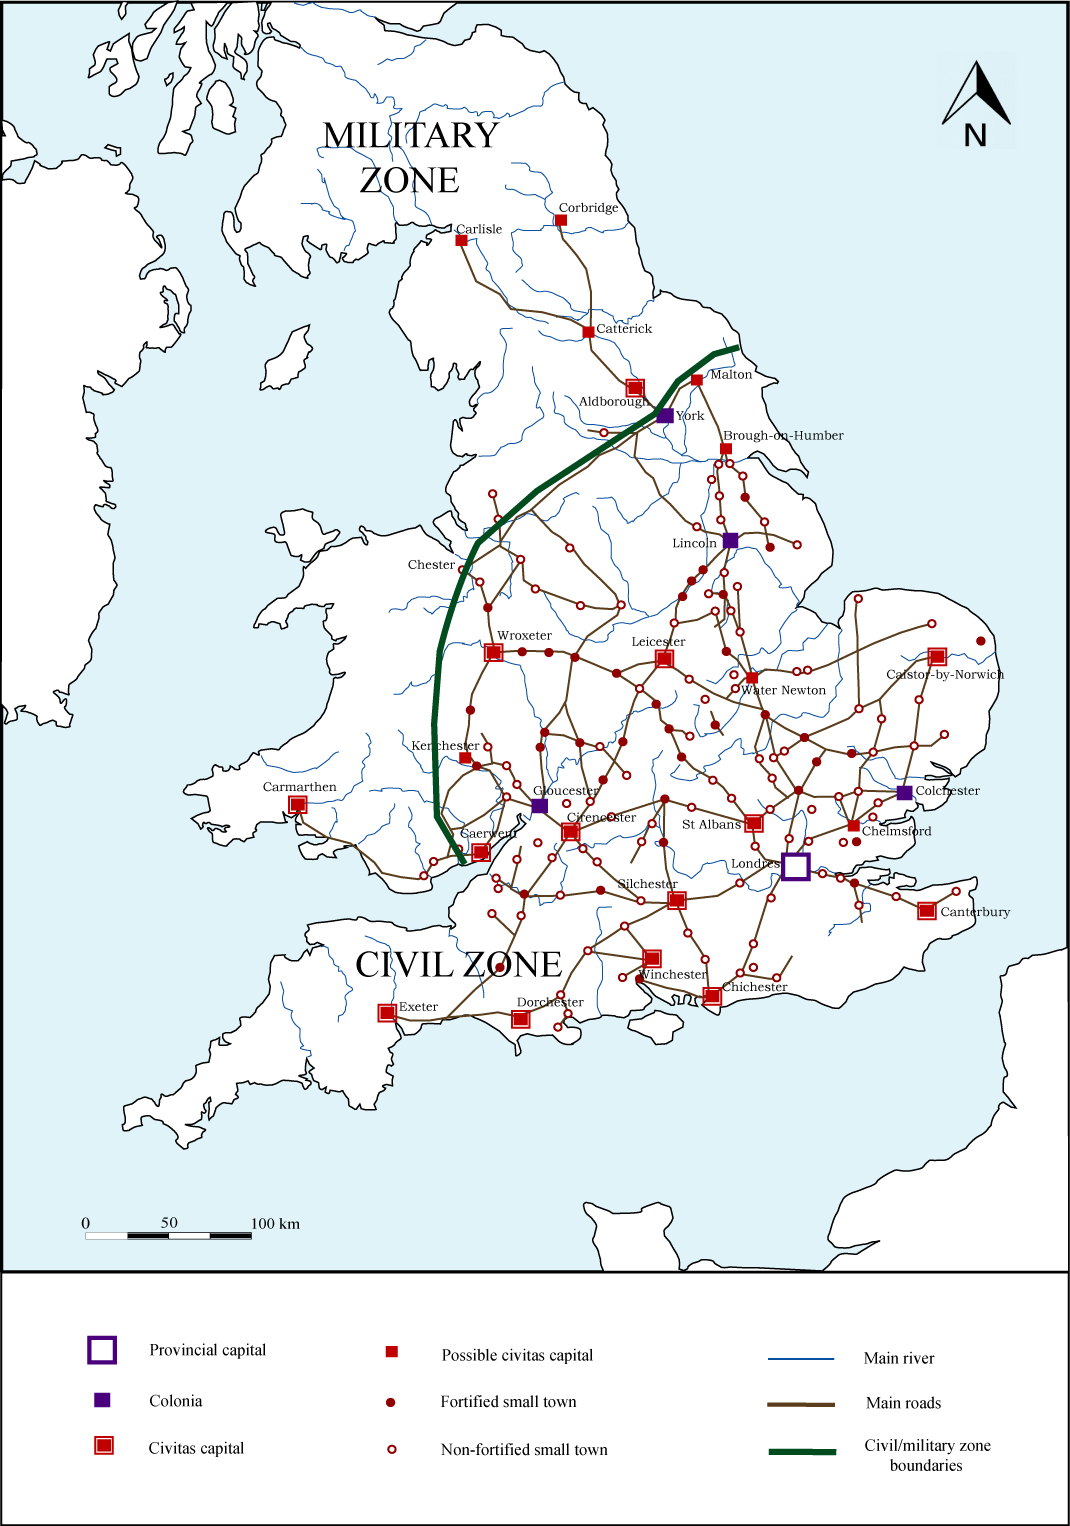
\includegraphics[width=\linewidth]{figures/rayer_Fig1.jpg}
		\caption{Distribution of towns and "small towns" according to current research. Illustration made by the author.}
		\label{fig:Rayer_Fig1}
	\end{figure}

%\section{“Small towns” and “\textit{vici}” in Northern Britain: terminological issues}

The\marginnote{“Small towns” and “\textit{vici}” in Northern Britain: terminological issues} incorporation of Britain into the Roman Empire led to the development of a particular settlement network in the region. The range of settlement types in northern Britain is immense: different types of sites are observed, with a multitude of sizes, origins, morphologies, and functions (Fig. \ref{fig:Rayer_Fig2}). Some settlements present urban or semi-urban characteristics, and are well developed, with a sizeable population, and evidence for industrial and/or commercial activities. Others were more agricultural in character, defined as farming communities or rural villages \parencites{Hingley_1989}{James_2001}{Jones_1991}{Wacher_1995}. Two main categories of sites emerge from research in the study area: the "small towns" and the "military \textit{vici}" \parencites{Rodwell_1975}{Sommer_1984}{Sommer_2006}{Wacher_1995}. This section reviews these various categories of settlements and their attributes, and the problems inherent to this classificatory scheme. 

	\begin{figure}
		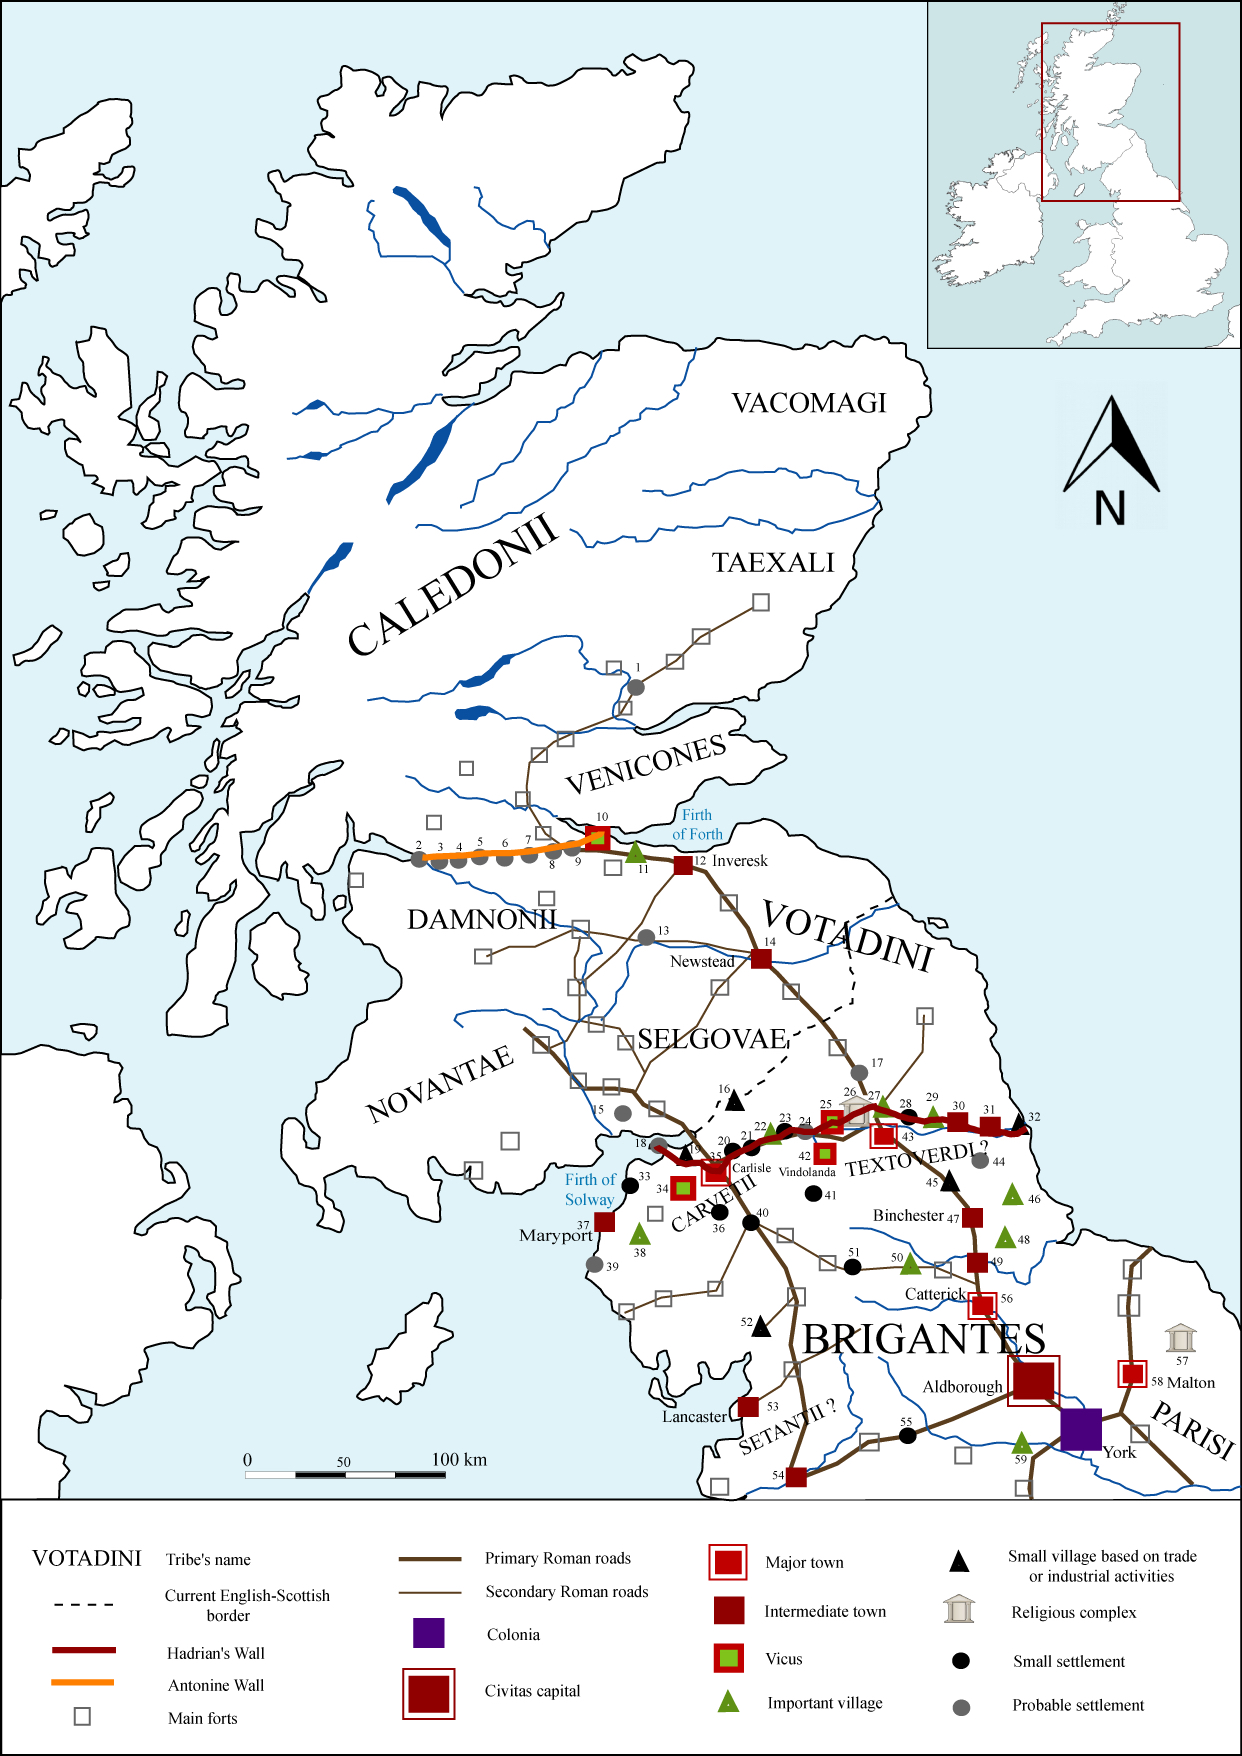
\includegraphics[width=\linewidth]{figures/rayer_Fig2.jpg}
		\caption{General map of Roman towns and civil settlements in Northern Britain. Illustration made by the author.}
		\label{fig:Rayer_Fig2}
	\end{figure}

%\subsection{Small towns}

The\marginnote{Small towns} term “small towns” refers to a form of settlement, subordinated to a \textit{civitas} capital. This expression is not sufficient to understand and describe Roman settlements, since it only encompasses cities and town with urban character and eludes all those whose functions were exclusively rural, like villages and hamlets \parencites{Favory_2012}{Rivet_1975b}{Smith_1987}{Todd_1970}{Wacher_1995}. Although the term “urban” appears as a qualifier for “city” or “town” sites, it has experienced a rather broad definition in archaeological practice, and scholars tend not to give specific definitions regarding the word “urban” \parencite[29]{Renfrew_2008}. There are several unifying features, common in all definitions: an extensive settlement size occupied permanently with evidence of internal organization and social distinction in the architecture; a suggested administrative significance; a large diversity of political and social buildings and institutions; a high level of economic activity, with some industrial productions in specialized areas; the possession of a market or fair functions, connected most of the time to an important road, river or sea, etc. \parencite[29]{Renfrew_2008}. On the contrary, non-urban settlements indicate sites which, by their activity or extend, do not possess the characteristics of urban settlements. There are several types, which can vary in size: villas, non-villa settlements that include single farms, small hamlets (two or three farms), large hamlets (four to six farms) and finally villages that embrace seven farms or more \parencite[76]{Hingley_1989}. These non-urban sites are some form of nucleated settlements (except villas and single farmsteads), involving a community and subordinated to a \textit{civitas}. I argue that these non-urban sites should be further considered in analyses of settlement patterns, given that both hamlets and small villages were quite common features of the inhabited landscape of Britannia \parencites[cf.][]{Hingley_1989}{Hanley_2000}. 

At the Oxford conference held in 1975 on the theme of the small towns of Roman Britain, \textcite[1]{Rodwell_1975} defined a “small town” in these terms:

\SetBlockThreshold{1} 
\blockquote{\textit{If we remove at one end of the settlement-scale coloniae, municipia and civitas capitals, and at one other end of the scale, villas, farmsteads and small villages which occupy an area of only a few hectares, we are left with a substantial residue of sites to which terms like “small town”, “minor town” and “large village” have been applied.}\footnote{\textcite[1]{Rodwell_1975}}}

Moreover, as Rivet stressed at the same conference, the term “small” is misleading as it is not a question of size in any classification since some settlements, better called “subordinate town” or “minor town” according to him, can exceed in size some major cities and \textit{civitas} capitals \parencite[111]{Rivet_1975b}.
In addition, Malcolm \textcite[115]{Todd_1970} asks a vital question for an important reflection on terminology issues: 

\SetBlockThreshold{1} 
\blockquote{\textit{The first problem to be encountered is one of terminology, for the minor settlements are by no means a homogeneous group. The portmanteau term 'small towns', under which they are commonly considered, often in the same context as the large urban centres, seems immediately to beg a vital question. To what extent were any of these settlements towns?}\footnote{\textcite[115]{Todd_1970}}}


In France, archaeologists use the term, \textit{agglomeration secondaire}, to talk about this type of settlements. It is also a very neutral and globalizing expression, encompassing sites with urban character, echoing Rodwell and Rowley’s definition, but which also includes small villages and hamlets into the range of nucleated settlements \parencite[18]{Mangin_1986}. As such, it may be preferable to use more neutral terms such as “minor settlements” or "civil settlements" rather than “small towns”, more consistent with the archaeological reality.

	\begin{figure}
		\includegraphics[width=\linewidth]{figures/rayer_Fig3.jpg}
		\caption{List of sites under study}
		\label{fig:Rayer_Fig3}
	\end{figure}

%\subsection{Military vici}
	
Civil\marginnote{Military vici} settlements near military forts are usually associated with the name of \textit{canabae} or military \textit{vici}. Many epigraphic evidences mention these two Latin terms in the Roman world, which causes some complications \parencite[for this debate, see][]{Tarpin_2002}. Most of the settlements in northern Britain are called \textit{vici} in English literature \parencites[cf.][]{Salway_1965}{Sommer_1984}{Sommer_2006}. This term is now the subject of many debates about its definition, nature and characteristics \parencite{Tarpin_2002}. However, most evidence of the use of this word comes from civilian contexts, so it seems dangerous to use it as a generic term for several types of realities \parencites[42--43]{Favory_2012}{Tarpin_2002}.	
	
No Latin author used the term \textit{vicus} to refer to settlements near forts or in a military context \parencites{Birley_2009}{Tarpin_2002}. The Latin references discussing the multiple meanings of the term vicus are usually found in the writings of Caesar (\textit{De Bello Gallico} I, 5), Varro (\textit{De Lingua Latina} V, 160), Festus (\textit{De Significatione Verborum} XIX) and Isodore of Seville (\textit{Etymologiae} XV, 2), among others. But this term should not be considered as some sort of settlement with a very different status or an urban neighbourhood \parencite[10]{Leveau_2002}; instead, it can be almost unanimously applied to any settlement, particularly those relating to structures adjacent to a Roman fort or military structures. Nevertheless, as \textcite[19]{Birley_2009} emphasized, this term could have been applied to a civil settlement associated with a fort, whose legal status was special, or to define a very specific geographical area that was not under the military authority during a period of time. This was likely the case at Vindolanda \parencite[1700]{RIB_1965}. Therefore, it seems misleading to designate all forms of settlements as a \textit{vicus}, or a military \textit{vicus}, if no inscription mentions it.

Very few studies have been conducted on this type of settlements and they are not included in the various works on “small towns” \parencites[e.g.][]{Jones_1990}{Todd_1970}{Wacher_1995}. Although they are not “urban sites”, vici belong to a type of civil settlement, with their own origins, morphologies, functions and chronologies. These sites do not appear on any general map regarding "small towns" \parencite[e.g.][156]{Jones_1990} since they are not considered as purely "urban" in character. In a comparison between the distribution maps of nucleated settlements within the province of Britannia, the contrast between the North and South is quite striking (see Fig. \ref{fig:Rayer_Fig1}).

Thus, the current vision of the distribution of small towns in Northern Britain during Roman times seems inaccurate. Whereas the southern regions appear actually more urbanised, with a dense network of cities and small towns, the north is not deprived of civilian infrastructures and minor settlements. Following \textcite[8]{Branigan_1980}, I would argue that some “\textit{vici}” could be considered as some forms of primary urban development.

%\section{'Small towns' network: diversity of development, internal morphology and functions}

%\subsection{Origins and development}

In\marginnote{'Small towns' network: diversity of development, internal morphology and functions -- Origins and development} the northern part of the province, it is accepted that the vast majority of “small towns” have grown in connection with the military activities and the progress of Roman troops \parencite[9]{Burnham_1990}. 
These settlements follow defence systems and the layout of various campaigns from the end of the \nth{1} century\AD. The development of these settlements in urban centres depends on multiple factors such as economic or cultural expansion, related to trade or crafts for instance, or the presence of an important religious centre \parencites[9]{Burnham_1990}[5--6]{Frere_1975}. However, discussions remain focused on the importance of military activities in the setting of Roman settlements, at the expense of economic, cultural, or chronological aspect \parencite[for this debate, see][7--8]{Burnham_1990}. 
A few sites from a military context, nonetheless, became developed enough to achieve a high status or an urban form, such as Carlisle \parencite{McCarthy_2002}, Corbridge \parencites{Bishop_1988}{Hodgson_2008} and Malton \parencites{Wenham_1974}{Wilson_2006}.

It is considered at present that at least a third of identified “small towns” are known to have developed from or near a pre-conquest Iron Age site, mainly in the south-eastern part of the province \parencite[20]{Wacher_1995}. The main forms of settlements that characterise the north of England and Scotland in prehistoric times are generally identified as fortified farms, isolated from each other, brochs –Scottish drystone hollow-walled structures– or souterrains –underground structures– \parencite[61]{Jones_1990}. Therefore, these societies with a more dispersed settlement pattern have not developed into many major centres, with some exceptions. The settlement of Newstead, built near a Roman fort and the hillfort of Eildon Hill North, is one of the examples of civilian settlement that grew in the presence of an Iron Age administrative centre \parencite{Hunter_2012}.

There are also some cases where settlements show no prehistoric origin or no relation to any Roman military presence. This could reflect a spontaneous development by some Romans or some indigenous community, as illustrated by the site of Sedgefield \parencite{Durham_2010} and Faverdale \parencite{Proctor_2012} in the \textit{Brigantes} territory, a so-called ‘Celtic’ tribe settled in northern England. These unplanned developments can be explained by the presence of major communication routes or the presence of raw materials that would allow the installation of a community developing around industrial commercial or administrative activities \parencite[5--6]{Frere_1975}. However, their origins are more complicated to understand since they do not appear to be the result of a deliberate act of foundation \parencite[55]{Jones_1991}.

The formation of the northern “small town” network in Britannia can be explained by several factors. Areas of high concentration of settlements tend to be the most militarised places: the two walls (the Hadrian and Antonine Walls), the defensive line across the Firth of Forth, the area called “Western Sea Defences” on the Solway Firth, and along two major roads linking the northern and southern parts of the province, mainly in the east on Dere Street. The road network (prehistoric tracks still in use until the creation of new Roman roads) and maritime and/or inland waterways are also deciding factors when creating a settlement \parencite[256]{Mattingly_2006}. The study of town’s morphology and street network allows to highlight the roles of some roads, rivers or streams in the development of settlements \parencite[203]{Petit_1994a}. The most important of these roads is Dere Street, crossing the entire northern part of the province between \textit{Eboracum} (York) and \textit{Veluniate} (Carriden). Another major pathway is the Stanegate, stretching from \textit{Luguvalium} (Carlisle) to \textit{Corstopitum} (Corbridge). The various constraints and benefits of the physical environment of the region can also highlight some concentrations or deserted areas. Finally, the political context, leading to the redistribution of some parts of the province, and new socio-economic conditions had a considerable influence on the development of urban centres or minor settlements \parencites[11]{Branigan_1980}[12]{Burnham_1990}.

%\subsection{Internal morphologies}

The \marginnote{Internal morphologies} total expansion of civil occupation on these sites is generally poorly understood due to the lack of extensive research. However, it is possible to deduce it from various elements such as the presence of fortifications or by geophysical surveys. Catterick is a particularly well-known example where a wide ditch had surrounded the main area of occupation at the end of the \nth{3} century\AD, covering a surface of approximately \SI{6}{\hectare} \parencite[57]{Hartley_1988}. Thereby, we can organize the fifty-nine “small towns” under study into three categories according to their estimated total area:

\begin{enumerate}
	\item Large settlements whose area exceeds \SI{20}{\hectare}, such as Carlisle, Corbridge, Sedgefield, or Malton (see Fig. \ref{fig:Rayer_Fig4}-\ref{fig:Rayer_Fig9}). Their full extension is generally not known but some appear to exceed in size several civitas capitals.
	\item Eighteen sites of medium size, between 10 and \SI{20}{\hectare} are actually known, such as Inveresk, Newstead, Birdoswald, Housesteads and Vindolanda.
	\item Finally, the remaining settlements, thirty-five, are smaller than 10ha. These are, in most cases, sites whose occupation is relatively short or whose economic influence is modest or only local. 
\end{enumerate}

The development of a Roman civil settlement in the northern part of the province is generally linear, alongside a main axis \parencites[234--235]{Burnham_1994}[97]{Sommer_2006}. More sophisticated plans could emerge from this type of extension by adding new parallel or perpendicular streets to the main axis, as seen in Birdoswald \parencite[100]{Biggins_1999} and Chesters \parencite[52]{Joseph_1951}. Sometimes, civil settlements could also grow at road junctions, or near a river crossing such as Newstead \parencite{Hunter_2012}. It is however important to emphasize the small number of grid plans, at Catterick \parencites{Wilson_2002a}{Wilson_2002b} and Malton \parencite{Wenham_1974} for instance. These few examples of internal street planning, probably introduced from the beginning of the occupation, contrast with the haphazard plans and spontaneous developments on most sites.

The vast majority of buildings found in the settlements under study are simple timber or stone structures, generally rectangular in shape, 
called “strip-buildings” or “strip-houses” \parencite[232]{Burnham_1994}. 
Their size can vary significantly, but most structures are relatively large, sometimes exceeding \SI{50}{\metre\squared} \parencite[66]{Osborn_2006}. 
Some probably had several pieces for the practice of trade or industrial activities: it is most likely the case in Maryport for some large structures \parencite[128]{Biggins_2004a}, for example. Some houses also have a room in front of the building, suggesting the installation of a portico, as is seen at Housesteads for instance \parencite[67]{Osborn_2006}. It is also possible to find more complex and elaborate structures, as shown in the example of the “Town House” in Malton \parencite[37]{Wenham_1974}. 
However, regardless of the growing interest in Roman settlements, internal buildings have rarely drawn attention, despite the abundance of information available concerning the types and methods of construction and the use of different materials \parencite[35]{Burnham_1988b}. 

Alongside these residential buildings, many types of buildings with various functions can be encountered:

\begin{itemize}
\item \emph{Official buildings} such as administrative buildings, are rare. No civic centre has been found at the present time and a single structure found at Carlisle could be likened to a potential forum \parencite[76]{McCarthy_2002}. 

\item \emph{Buildings with economic responsibilities} can be identified in various settlements. Houses themselves have craft or trade related functions as seen above, through the presence of workshops at the front of some buildings. Some marketplaces are also possible: at Birdoswald \parencite[176]{Biggins_2004b} and Newstead \parencite[84]{Hunter_2012} for example.

\item \emph{Religious and cultural places} have also been identified. The most common and distinctive places of worship are so-called Romano-Celtic temples, with square and octagonal plans \parencite[53]{Burnham_1988b}. Entertainment buildings such as possible theatres and amphitheatres can also be found in this part of the province, but these are extremely rare \parencite[see for instance][]{Neighbour_2007}. 

\item \emph{Public amenities} can also be seen but more difficult to identify: street network is evident on many sites, sewers are reported, bridges, and fords are also attested. Water supply is difficult to define but on many cases, wells are the only visible remains.
\end{itemize}


%\subsection{A variety of functions}

It\marginnote{A variety of functions} is clear that many settlements owe their origin and prosperity to some predominant functions (administrative, religious or economic). Most sites have also been able to acquire one or more new functions over time, resulting from their geographical position, requests generated by the civilians and the army, or from various territorial policies \parencite[289--290]{Mattingly_2006}.

The most represented activities on all settlements are related to economy, regardless of the degree of development of these sites. The first forms of these activities are linked to agricultural exploitation, raw materials, and industrial production \parencite[34--35]{Sommer_1984}. These primary and secondary sectors are almost omnipresent on all sites. The archaeological evidence from thirty sites confirmed agro-pastoral activities and/or exploitation of natural resources (stone, wood etc.). Forty sites also reveal activities related to the production of manufactured objects (see Fig. \ref{fig:Rayer_Fig4}--\ref{fig:Rayer_Fig9}). 
Only one inscription mentioned craftsmanship: a goldsmith at Malton \parencite[712]{RIB_1965}.

The main industrial activities represented in the archaeological record are related to pottery and metal production (see Fig. \ref{fig:Rayer_Fig4}--\ref{fig:Rayer_Fig9}). Other activities, far less represented and more widely dispersed throughout settlements, can also be found: manufacture of woollen clothing, leather and textile, wood, bone or stone manufactures, etc. \parencites[148]{Clack_1982}[35]{Sommer_1984}[for the example of a workshop of Roman sculptures at Carlisle, see][90]{McCarthy_2002}. The relationship between a fort and a surrounding settlement was a partnership; the fort’s garrison provided a demand and the civilians supplied the goods and services required \parencite[85]{Bidwell_2007}. Therefore, they were centres for industry and trade (on a modest scale), including land, sea and river trade, acting as sources and markets for goods. Evidence of workshops, marketplaces and possible port remains can be encountered in this part of the province and the Vindolanda tablets give us precious information on both imported and exported goods \parencites{Bowman_2008}[69]{Osborn_2006}.

Few settlements had a purely religious function. Only five sites possessed one or more places of worship. Religious buildings are similar to small temples or shrines of Romano-Celtic traditions. It is also important to note that these structures were generally not monumental and were relatively small in size. Some exceptions can be found at Corbridge \parencite{Hodgson_2010} and Carlisle \parencite[83]{McCarthy_2002}. Only two religious complexes were identified: Carrawburgh \parencite{Breeze_1972} and West Heslerton \parencite{Halkon_2013}, which seemed to be of small dimensions.

Finally, the close link between the settlements and forts makes it difficult to understand the internal organization of these sites \parencite[22]{Sommer_1984}. However, particular status is attested in a few cases. The executive power could be represented by some elected leaders referred as \textit{magistri vici} \parencite[found at Old Carlisle;][899]{RIB_1965} or by some magistrates or imperial officers such as \textit{curators vicanorum} at Vindolanda \parencite[1700]{RIB_1965}. Administrative functions are well highlighted in some sites by epigraphic mentions, but also thanks to the presence of \textit{cursus publicus} buildings (relay points and transportation service of the Roman Empire) found at Chesters for example \parencite{Hodgson_2009}.

%\section{A classification of Roman civil settlements in Northern Britain: a new perspective?}

The\marginnote{A classification of Roman civil settlements in Northern Britain: a new perspective?} reconsideration of the available archaeological evidence carried out above can be synthesised in a general typological table covering all sites under study (Fig. \ref{fig:Rayer_Fig4}--\ref{fig:Rayer_Fig9}), allowed to classify the settlements into different categories. Three main categories stand out clearly: settlements with urban features, transitional sites between major towns and small rural villages, and lastly, some very small agglomerations with apparently little influence on the surrounding landscape.

The first category consists of some settlements with urban character and several dynamic sites, which include two subcategories: major towns and intermediate towns/\textit{vici}.

\begin{itemize}
\item \emph{Major towns} have a pronounced urban character, a major extension, multiple functions and infrastructures, and their status could change over time to rise to the rank of a civitas capital (\parencite[at Carlisle;][933]{RIB_1965}. This category includes only four of the sites under study: Carlisle, Corbridge, Catterick and Malton. These towns had a considerable influence on a regional scale and a large extension; the area they covered is generally exceeding \SI{20}{\hectare}. They also had a particularly pronounced urban character, usually shown through grid plans, architectural forms and a large variety of public infrastructures \parencites{Bishop_1988}{McCarthy_2002}{Wilson_2002a}{Wilson_2002b}{Wilson_2006}.

\item \emph{Intermediate towns and \textit{vici}} (as mentioned on inscriptions) are dynamic settlements of a relative importance, with multiple functions and some public amenities. Thirteen settlements are gathered in this category: Inveresk, Newstead, Benwell, Wallsend, Maryport, Binchester, Piercebridge, Lancaster, Ribchester, and four \textit{vici}: Carriden, Housesteads, Old Carlisle and Vindolanda. These sites, except perhaps Piercebridge \parencite{Cool_2008} during its first years of occupation, are mainly related to military activity. They are dynamic and attractive centres in the network north of the province, which survived a century or two, sometimes three in some cases. Their extension is generally smaller than major towns, extending mainly from \SIrange{10}{20}{\hectare}. In most cases, these civil settlements do not have monuments characterising a Roman city such as \textit{forum}, temples, or entertainment structures. The major difference between these sites and major towns is the internal organisation that follows a more linear development around a main axis rather than a grid plan \parencites{Birley_2009}{Crow_2004}{Osborn_2006}{Sommer_1984}{Sommer_2006}{Wilson_1997}. Many functions are also present, but they are less diversified: several types of industrial production and economic activities may have been conducted on multiple sites although they are rarely identified simultaneously. Official and religious functions may also be present but are more discrete. 
\end{itemize}
Secondly, we can distinguish many sites which make the transition from major towns to small rural villages. This category includes important villages, small villages axed on one commercial or productive activity and religious complexes:

\begin{itemize}
\item \emph{Important villages}, whose surface is sometimes considerable, but do not feature any official or public buildings (except for some rare cases). These settlements have a smaller influence on the territory and primary and secondary sectors prevailed. These are above all economic centres whose extension can sometimes be even larger than some \textit{civitas} or towns, at Sedgefield for example \parencite[264]{Burnham_2007}. They are mainly characterised by the preponderance of agricultural and small scale industrial activities and their very modest civil architecture. They usually have an internal layout based on a linear extension along a main road and around which some streets could be added \parencites[see e.g.][]{Hodgson_2009}{Proctor_2012}{Sommer_1984}{Sommer_2006}{Wilmott_2001}. These villages are: Cramond, Birdoswald, Chesters, Rudchester, Papcastle, Sedgefield, Faverdale, Greta Bridge, and Newton Kyme.

\item \emph{Small villages axed on one productive or commercial activity}, whose expansion is even further reduced, usually display a single dominant economic function (trade or crafts). These are mainly Netherby and South Shields \parencites{Cleary_1997}{Snape_2010} for the commercial function, and Burgh-by-Sands, Lanchester and Watercrook \parencites{Breeze_2009}{Potter_1979} for industrial activities. However, it is important to note that the distribution of these sites in a particular category may seem arbitrary when the lack of large-scale excavations did not identify traces of any other activities.

\item At last, in this second category, we found the \emph{religious complexes} where the unique function is one of religious significance. These settlements usually have several temples or shrines, and are places of pilgrimages. Only two sites can be identified as such in the area under study: Carrawburgh \parencite{Snape_1994a} and West Heslerton \parencite{Powlesland_1998}. The internal organisation of these settlements is poorly understood and their distribution does not seem to follow any particular model.
\end{itemize}

Finally, the last types of settlements on the area are very small agglomerations with low influence on the territory, comprising minor and probable settlements.

\begin{itemize}
	\item \emph{Minor or small settlements} are similar to present villages and hamlets, with only some agro-pastoral functions and a very local influence. Their size is very small, never exceeding 5 or \SI{10}{\hectare}. No public structures are found within these sites. Domestic buildings are very simple and the use of stone is rarely attested, except for some foundations. We can find in this category: Stanwix, Castlesteads, Carvoran, HaltonChesters, Beckfoot, Old Penrith, Brougham, Whitley Castle, Bowes, and Ilkley \parencites[see for instance][121]{Casey_1998}[124--127]{Hodgson_2009}.
	\item \emph{Probable settlements} are sites where lack of information (see Fig. \ref{fig:Rayer_Fig4}-\ref{fig:Rayer_Fig9}) and/or excavations do not allow their secure identification or classification in any of the categories set out above. There are seventeen of these cases in the corpus of sites under study: Cargill, Old Kilpatrick, Bearsden, Balmuildy, Cadder, Croy Hill, Castlecary, Camelon, Mumrills, Easter Happrew, Birrens, Risingham, Bowness-on-Solway, Great Chesters, Moresby, and Chester-le-Street. They are largely found in the north of the survey area, in Scotland, and mainly along the Antonine Wall. 
\end{itemize}

It is hard to define whether the discovered buildings represent civil buildings or military annexes, since the nature of the remains is poorly understood in the absence of large-scale excavations. Moreover, other sites have not been selected in this study because of limited available data. This is particularly the case at Auchendavy, Bar Hill on the Antonine Wall, or Ravenglass, Kirkby Thore and Ambleside, south of the Hadrian Wall. Such withdrawal is due to incomplete data or remaining elements that can accurately certify the possible presence of a civilian settlement. At Auchendavy for example, only two engraved stones may refer to civilians: a fifteen years old child \parencite[2182]{RIB_1965} and a woman \parencite[2183]{RIB_1965}, which is not sufficient in absence of any other elements indicating a possible settlement.
	
%\section{Conclusion}

This\marginnote{Conclusion} study, conducted on the so-called Roman “small towns” in northern Britain, gives an overview of current knowledge on the subject and identify the principal difficulties associated with the study of settlement patterns, starting with the terminology itself. The first significant conclusion is the considerable imbalance of knowledge and data availability across the study area. The scarcity of archaeological evidence from some sites, areas or topics, does not enable to transcribe accurately the organisation of Roman civil settlements in northern Britain. Terminological issues in English literature between "small towns" and "military \textit{vici}" makes it very complex to understand networks of civil settlements, particularly in the northern regions of the province, which are usually regarded as purely military areas. Moreover, in the rural landscape, non-villa settlements are rarely considered for archaeological investigation, as \textcite[76]{Hingley_1991} pointed out; thus, rural settlement patterns are poorly understood. We need to conduct intensive studies on a number of individual areas in order to have a better insight into settlement hierarchy.

Nevertheless, after considering a comprehensive sample of civil settlements in this study, located in a supposedly military context, and the “small towns”, seen as purely civilian population centres, it is possible to observe certain similarities in their origins, forms, and functions. I argue that the current picture of town distribution in northern Britain is inaccurate and incomplete, since some types of settlements are systematically not taken into account. Indeed, as argued by \textcite[76]{Jones_1991}, where lays the demarcation between villages and small towns? Even though the southern regions appear as more urbanised, with a dense network of cities and “small towns”, the northern part of the province is not deprived of civilian infrastructure or population centres. The separation between a “military zone” in the north and a “civil zone” in the south appears therefore incorrect, at least from this perspective. The settlements encountered in northern Britain are indeed closely linked to military activities. However, they are part of a type of civil settlements that needs to be contextualised on a broader scale, because, the vast majority of sites in the south of the province are equally associated to various military activities or defence structures. Then, why did a division between equivalent settlements forms and patterns, only different because of development inequalities, occur? The portray of a strong military presence in the northern part of the province, frequently mentioned in ancient sources, could help explain the disparities between the interpretation of the north as more rural, and the south, more urbanised and rapidly demilitarised \parencite[291]{Mattingly_2006}.

The division between civil and military zones seems therefore imprecise, since no less than fifty-nine sites with various forms, functions, and statuses were studied over the entire area. It is a dense, organised and hierarchical network that does not differ significantly from the southern one, except in the fact that it is less urbanised. Therefore, I argue that the term “small town” should be replaced by a more neutral term, such as “minor settlement” or “civil settlement” to refer to all forms of nucleated establishments, ranging from the largest Roman town subordinated to a \textit{civitas} capital to a small hamlet consisting of few individuals. Finally, it is important to recall once again the difficulty of such studies, caused by lack of archaeological data and by the need to agree on a clear and unanimous terminology. There is therefore a growing need to break away from previous works to review the available data and an obligation to undertake further studies on a regional scale. \textcite[66]{Millett_2001} argued that we need to rethink some of the questions about urban and rural societies as our approaches were almost completely dominated by military questions. We need to reconsider the different categories we use to describe the sites and what characterised or constituted Roman urbanism. Many \textit{vici} have to be considered as “towns” as he explains: 

\SetBlockThreshold{1} 
\blockquote{\textit{These sites played a key role in parts of the province and many of us would not draw a far less firm distinction between army and civilians than their separate treatments suggest.}\footnote{\textcite[64]{Millett_2001}}}

New lines of research also need to be developed or completed, particularly on settlements distribution and morphology, urban-rural relations, the changing pattern of land use or the role of the Roman army in promoting or retarding the urban process \parencite[74--75]{Burnham_2001}. 
Lastly, it is important to remember that the interaction between Romans and local populations or the impact of the Roman administration on Iron Age organisation are questions that should also be addressed, since these can help us to understand the formation of the civil settlement network during Roman times.


\begin{myabstract}
\foreignlanguage{french}{%			
		L’enjeu de cette étude est de remettre en question la military zone et les modalités d’implantation des Romains dans la partie nord de la Grande-Bretagne en redéfinissant le terme small town (ou agglomération secondaire) et en reconsidérant les données archéologiques disponibles pour cette aire géographique. Ce travail dresse un bilan général de nos connaissances actuelles sur le sujet et identifie les faiblesses et diverses difficultés que comporte l’étude des réseaux d’habitats groupés. Il livre également un nouveau regard sur les agglomérations secondaires en Bretagne romaine et tente de proposer de nouvelles perspectives ou approches afin de comprendre les modalités d’implantation et l’occupation du sol à l’extrême nord de l’empire romain.
	}		
\end{myabstract}
\clearpage
\begin{figure}[!p]
		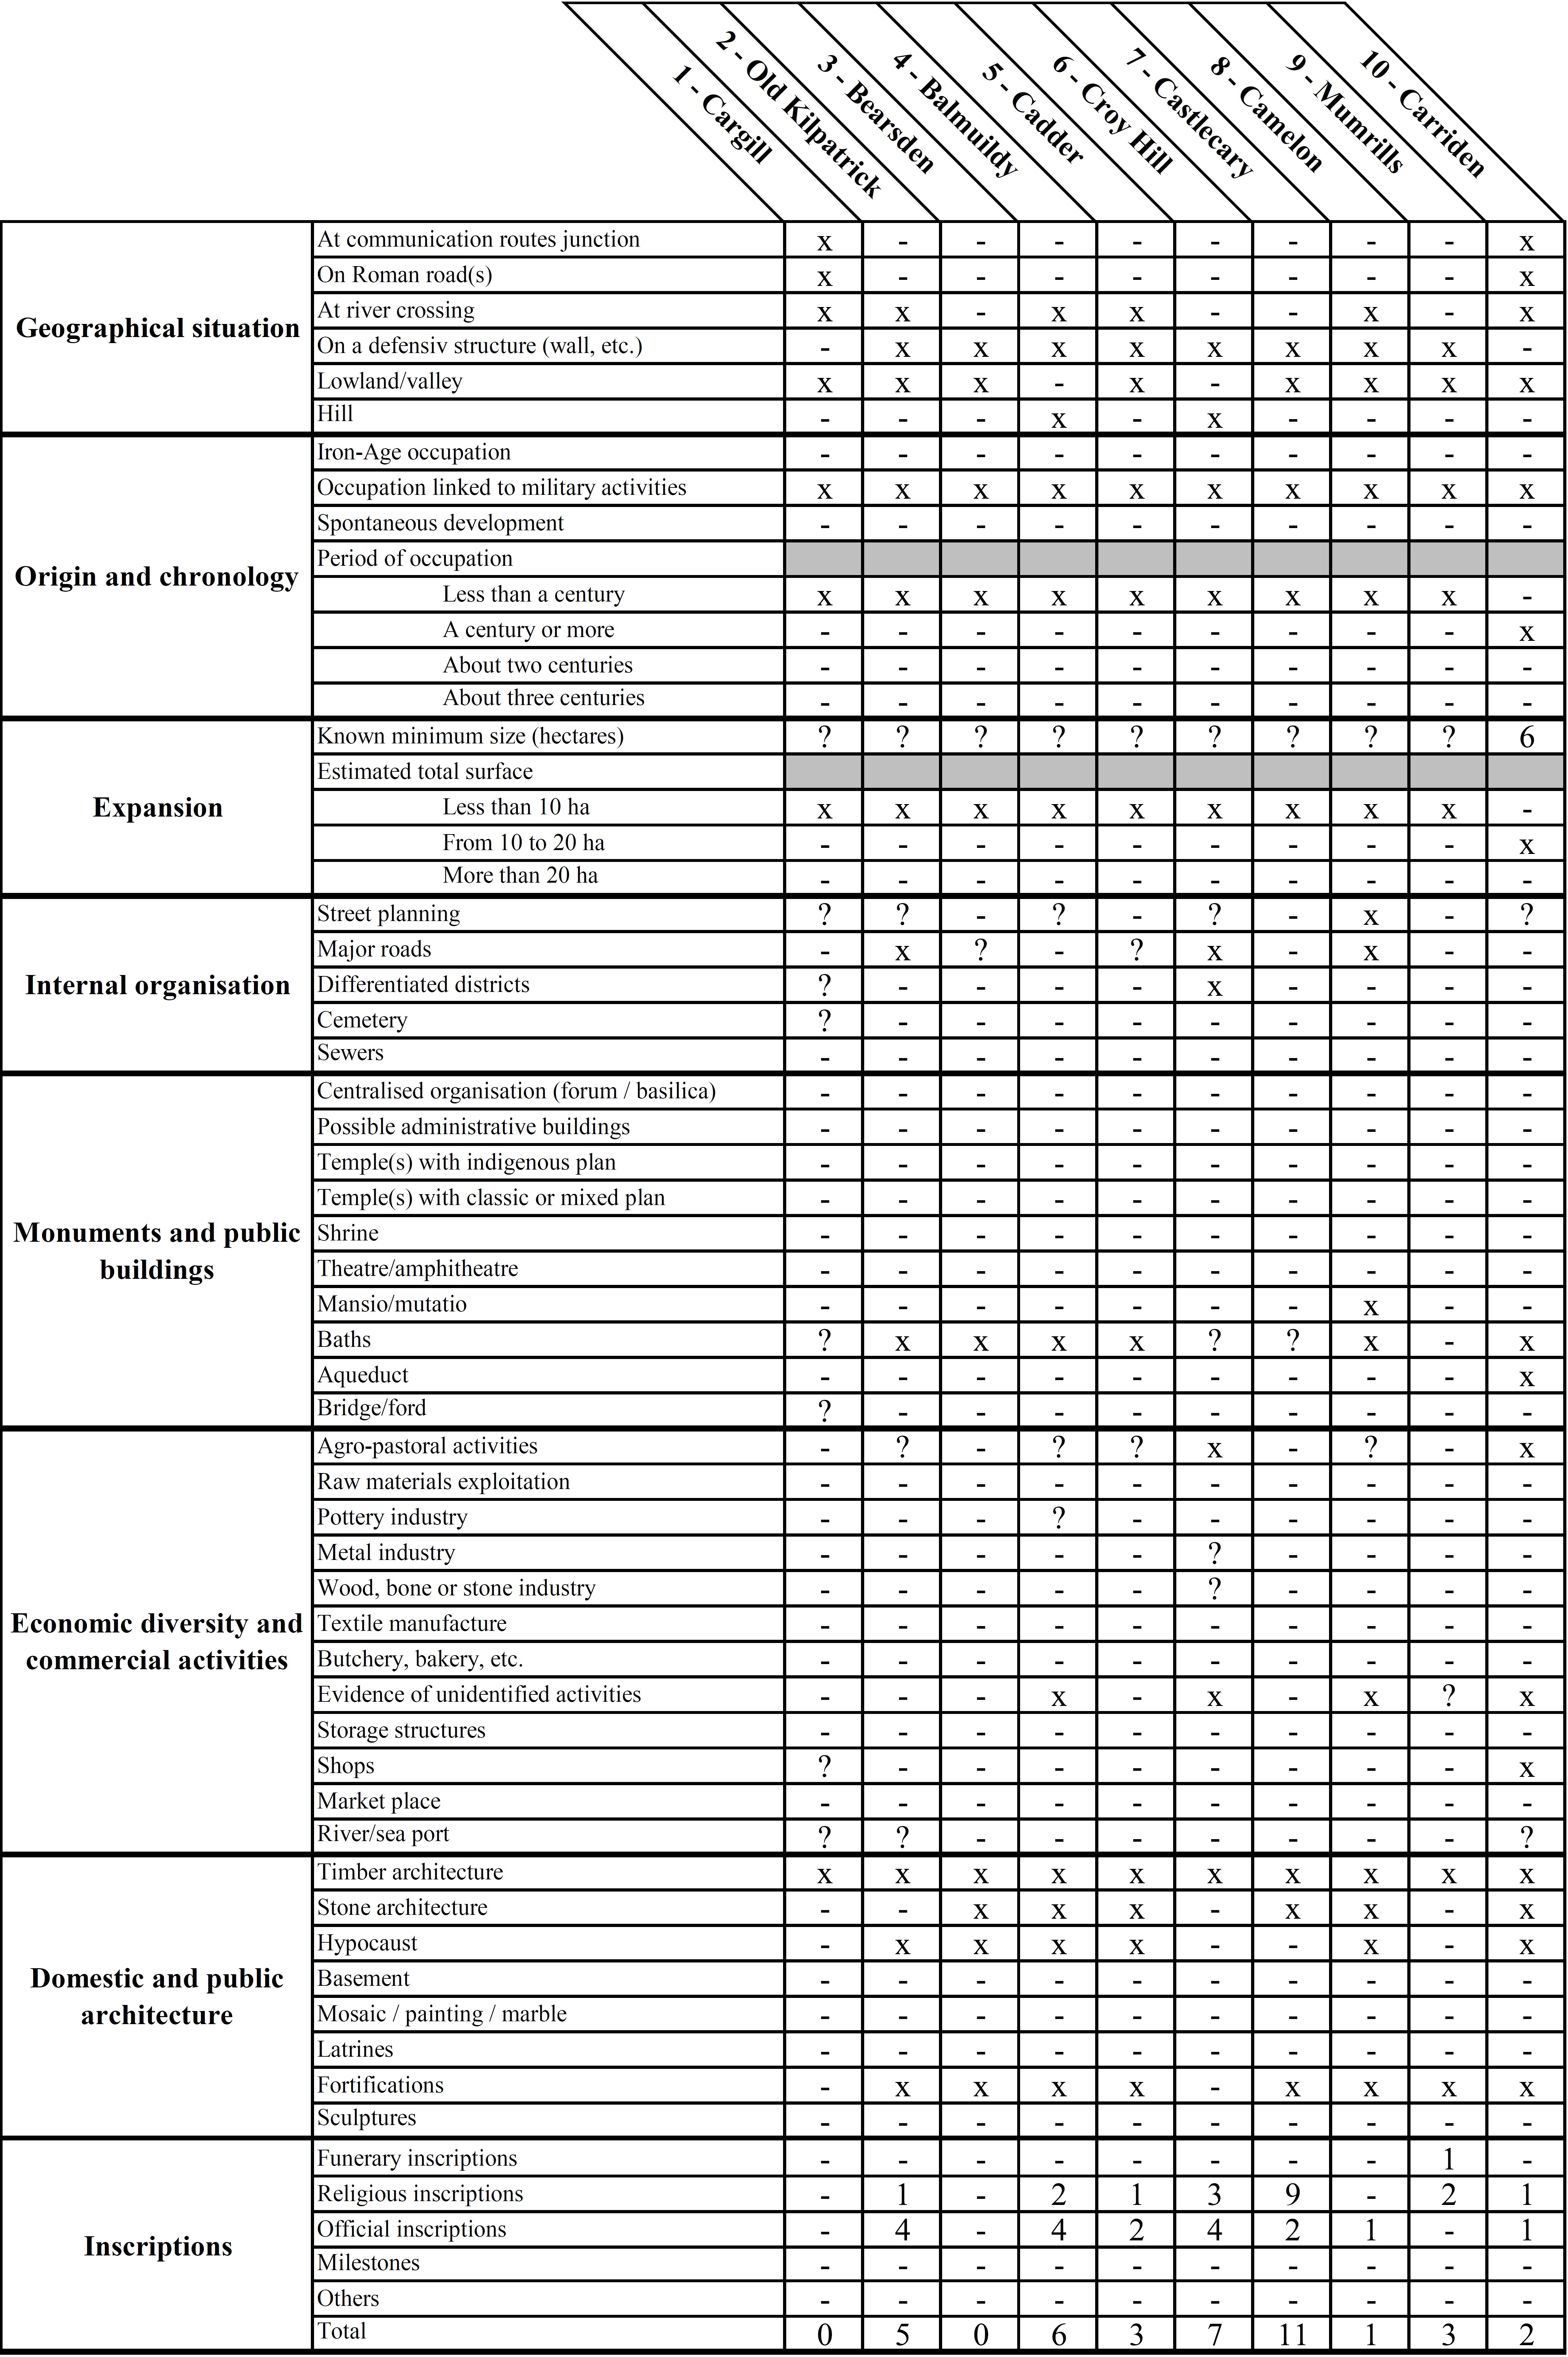
\includegraphics[width=\linewidth]{figures/rayer_Fig4.jpg}
		\captionof{table}{General typological table of civil settlements. Table made by the author.}
		\label{fig:Rayer_Fig4}
	\end{figure}
	
		\begin{figure}[!p]
			\includegraphics[width=\linewidth]{figures/rayer_Fig5.jpg}
			\captionof{table}{General typological table of civil settlements. Table made by the author.}
			\label{fig:Rayer_Fig5}
		\end{figure}
		
			\begin{figure}[!p]
				\includegraphics[width=\linewidth]{figures/rayer_Fig6.jpg}
				\captionof{table}{General typological table of civil settlements. Table made by the author.}
				\label{fig:Rayer_Fig6}
			\end{figure}
			
				\begin{figure}[!p]
					\includegraphics[width=\linewidth]{figures/rayer_Fig7.jpg}
					\captionof{table}{General typological table of civil settlements. Table made by the author.}
					\label{fig:Rayer_Fig7}
				\end{figure}
				
					\begin{figure}[!p]
						\includegraphics[width=\linewidth]{figures/rayer_Fig8.jpg}
						\captionof{table}{General typological table of civil settlements. Table made by the author.}
						\label{fig:Rayer_Fig8}
					\end{figure}
					
						\begin{figure}[!p]
							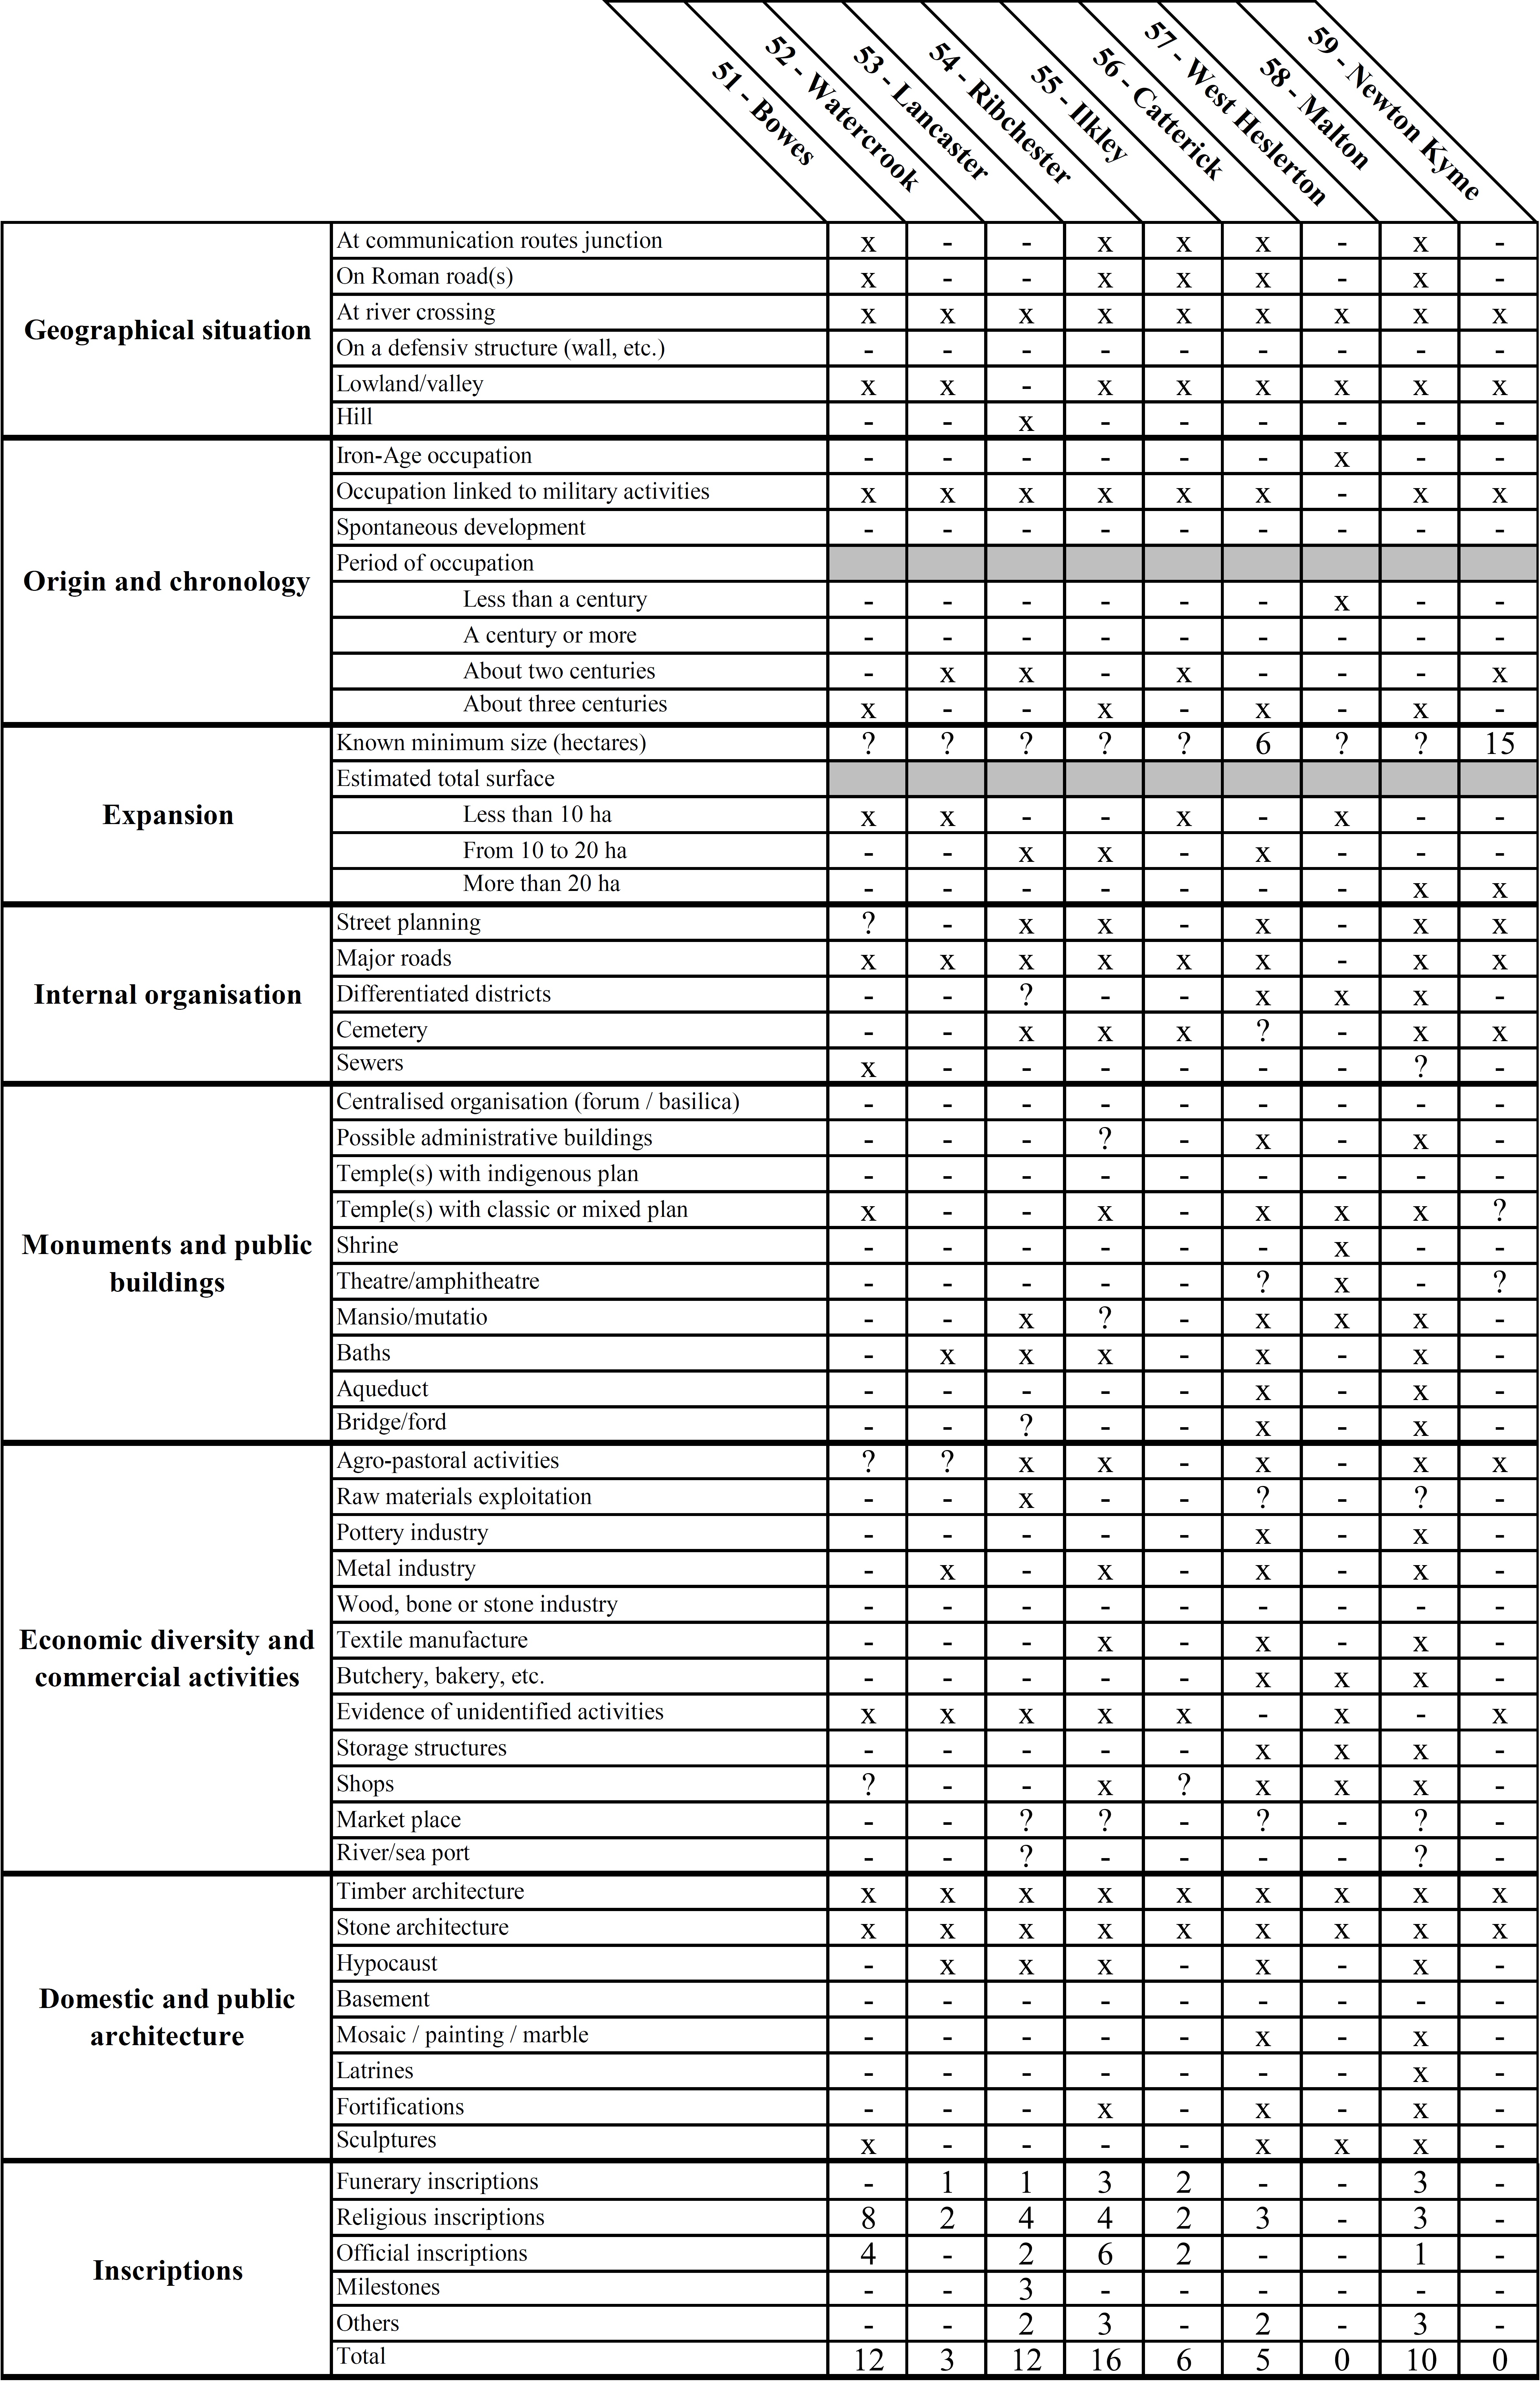
\includegraphics[width=\linewidth]{figures/rayer_Fig9.jpg}
							\captionof{table}{General typological table of civil settlements. Table made by the author.}
							\label{fig:Rayer_Fig9}
						\end{figure}	

\clearpage
\printbibliography[heading=subbibnumbered] 
\label{Rayer:lastpage}
%----------------------------------------------------------------------------------------
\closingarticle

